\section* {2.1. Нахождение положительных корней нелинейного уравнения методами простой итерации и Ньютона}


\subsection{Постановка задачи}
Реализовать методы простой итерации и Ньютона решения нелинейных уравнений в виде программ, задавая в качестве входных данных точность вычислений. С использованием разработанного программного обеспечения найти положительный корень нелинейного уравнения (начальное приближение определить графически). Проанализировать зависимость погрешности вычислений от количества итераций. 

{\bfseries Вариант:} 5
\begin{align*}
& cos(x) + 0,25x - 0,5 = 0 \\
\end{align*}

\subsection{Результаты работы}
\begin{figure}[h!]
\raggedright
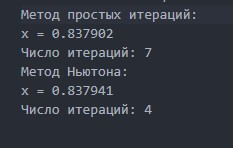
\includegraphics[width=.6\textwidth]{img1}
\end{figure}
\pagebreak

\subsection{Исходный код}
\lstinputlisting{include/2_1.cpp}
\pagebreak

\section* {2.2. Решение СНУ методами простой итерации и Ньютона}

\setcounter{subsection}{0}


\subsection{Постановка задачи}
Реализовать методы простой итерации и Ньютона решения систем нелинейных уравнений в виде программного кода, задавая в качестве входных данных точность вычислений. С использованием разработанного программного обеспечения решить систему нелинейных уравнений (при наличии нескольких решений найти то из них, в котором значения неизвестных являются положительными); начальное приближение определить графически. Проанализировать зависимость погрешности вычислений от количества итераций.   

{\bfseries Вариант:} 5
\begin{align*}
& \begin{cases}
x_1 - cos(x_2) = 1,\\
x_2 - lg(x_1 + 1) = 2
\end{cases}\\
\end{align*}

\subsection{Результаты работы}
\begin{figure}[h!]
\raggedright
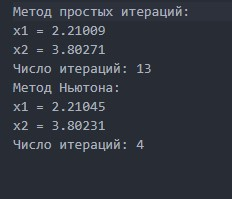
\includegraphics[width=.6\textwidth]{img2}
\end{figure}
\pagebreak

\subsection{Исходный код}
\lstinputlisting{include/2_2.cpp}
\pagebreak
